%%%%%%%%%%%%%%%%%%%%%%%%%%%%%%%%%%%%%%%%%%%%%%%%%%%%%%%%%%%%%%%%%%
%%%%%%%% ICML 2017 EXAMPLE LATEX SUBMISSION FILE %%%%%%%%%%%%%%%%%
%%%%%%%%%%%%%%%%%%%%%%%%%%%%%%%%%%%%%%%%%%%%%%%%%%%%%%%%%%%%%%%%%%

% Use the following line _only_ if you're still using LaTeX 2.09.
%\documentstyle[icml2017,epsf,natbib]{article}
% If you rely on Latex2e packages, like most moden people use this:
\documentclass{article}

% use Times
% \usepackage{times}
% For figures
\usepackage{graphicx} % more modern
%\usepackage{epsfig} % less modern
\usepackage{subfigure} 
\usepackage{bbm, bm, amsmath, amssymb, amsthm, mathrsfs}
\usepackage{booktabs, tikz, float}


% accent helper function
\usepackage{accents}
\DeclareMathSymbol{\fixwidehatsym}{\mathord}{largesymbols}{"62}
\newcommand\lowerwidehatsym{%
  \text{\smash{\raisebox{-1.3ex}{%
    $\fixwidehatsym$}}}}
\newcommand\fixwidehat[1]{%
  \mathchoice
    {\accentset{\displaystyle\lowerwidehatsym}{#1}}
    {\accentset{\textstyle\lowerwidehatsym}{#1}}
    {\accentset{\scriptstyle\lowerwidehatsym}{#1}}
    {\accentset{\scriptscriptstyle\lowerwidehatsym}{#1}}
}

% For citations
\usepackage{natbib}

% For algorithms
\usepackage{algorithm}
\usepackage{algorithmic}

% As of 2011, we use the hyperref package to produce hyperlinks in the
% resulting PDF.  If this breaks your system, please commend out the
% following usepackage line and replace \usepackage{icml2017} with
% \usepackage[nohyperref]{icml2017} above.
\usepackage{hyperref}


% Packages hyperref and algorithmic misbehave sometimes.  We can fix
% this with the following command.
\newcommand{\theHalgorithm}{\arabic{algorithm}}

% Employ the following version of the ``usepackage'' statement for
% submitting the draft version of the paper for review.  This will set
% the note in the first column to ``Under review.  Do not distribute.''
\usepackage[accepted]{icml2017} 

% Employ this version of the ``usepackage'' statement after the paper has
% been accepted, when creating the final version.  This will set the
% note in the first column to ``Proceedings of the...''
%\usepackage[accepted]{icml2017}


% The \icmltitle you define below is probably too long as a header.
% Therefore, a short form for the running title is supplied here:
\icmltitlerunning{Statistical Learning Final Project}

\begin{document} 

\twocolumn[
\icmltitle{Understanding Model Predictions via Influence Functions}

% It is OKAY to include author information, even for blind
% submissions: the style file will automatically remove it for you
% unless you've provided the [accepted] option to the icml2017
% package.

% list of affiliations. the first argument should be a (short)
% identifier you will use later to specify author affiliations
% Academic affiliations should list Department, University, City, Region, Country
% Industry affiliations should list Company, City, Region, Country

% you can specify symbols, otherwise they are numbered in order
% ideally, you should not use this facility. affiliations will be numbered
% in order of appearance and this is the preferred way.
\icmlsetsymbol{equal}{*}

\begin{icmlauthorlist}
\icmlauthor{Yundong Liu}{a,equal}
\icmlauthor{Yuze Liu}{r,equal}
\icmlauthor{Zhengyang Qi}{d,equal}
\icmlauthor{Ze Yang}{x,equal}
\end{icmlauthorlist}

\icmlaffiliation{a}{[yundongl@andrew.cmu.edu]}
\icmlaffiliation{r}{[yuzel@andrew.cmu.edu]}
\icmlaffiliation{d}{[zhengyaq@andrew.cmu.edu]}
\icmlaffiliation{x}{[zey@andrew.cmu.edu]}




% You may provide any keywords that you 
% find helpful for describing your paper; these are used to populate 
% the "keywords" metadata in the PDF but will not be shown in the document
\icmlkeywords{boring formatting information, machine learning, ICML}

\vskip 0.3in
]

% this must go after the closing bracket ] following \twocolumn[ ...

% This command actually creates the footnote in the first column
% listing the affiliations and the copyright notice.
% The command takes one argument, which is text to display at the start of the footnote.
% The \icmlEqualContribution command is standard text for equal contribution.
% Remove it (just {}) if you do not need this facility.

%\printAffiliationsAndNotice{}  % leave blank if no need to mention equal contribution
\printAffiliationsAndNotice{\icmlEqualContribution} % otherwise use the standard text.
%\footnotetext{hi}

\begin{abstract} 
In this paper, we reproduced \cite{koh2017}, using influence functions to trace a model’s prediction back to the training data. We carried out efficient implementations with \texttt{Tensorflow}, and demonstrated its performance \& applications on real-world datasets. 
\end{abstract} 
\section{Introduction}
\label{intro}

Consider a supervised learning problem with random input variable $Z=(X,Y)\in \mathcal{X}\times \mathcal{Y}$, following the joint CDF $F_{X,Y}$. $\{\bm{z}_i\}_{i=1}^n = \{(\bm{x}_i, y_i)\}_{i=1}^n$ are the realizations of the input variables, i.e. the training points. Assume we are estimating a hypothesis parametrized by $\bm{\theta} \in \Theta$. Let $\mathcal{L}(\bm{z}, \bm{\theta})$\footnote{We fold in any regularization terms in to $\mathcal{L}$.} be the loss for a point $z$. The desired parameter $\bm{\theta}(F_Z)=\mathrm{argmin}_{\bm{\theta} \in \Theta}\mathbb{E}\left[\mathcal{L}(\bm{z},\bm{\theta})\right]$ minimizes the expected prediction error. 

$\bm{\theta}$, as well as many other $\mathcal{M}$-estimators, falls in to a broader concept of \textit{statistical functional} \cite{nonp}, which is a mapping from the space of population cumulative distribution to some field. Given the training set, the empirical cumulative distribution $\fixwidehat{F}_Z$ is usually our best estimate to the true underlying population distribution. $\fixwidehat{\bm{\theta}} = \bm{\theta}(\fixwidehat{F}_Z)$, the plug-in estimator of the statistical functional, is obtained by solving empirical risk minimization problem.
\begin{align}\label{emprisk}
	\bm{\theta}(\fixwidehat{F}_Z)&=\underset{\bm{\theta} \in \Theta}{\mathrm{argmin}}\int\mathcal{L}(\bm{z},\bm{\theta})d\fixwidehat{F}_Z \notag\\[-5pt]
	&=\underset{\bm{\theta} \in \Theta}{\mathrm{argmin}}\int\mathcal{L}(\bm{z},	\bm{\theta})\frac{\partial}{\partial \bm{z}}\left(\frac{1}{n}\sum_{i=1}^n H(\bm{z}-\bm{z}_i)\right) d \bm{z}\notag\\[-5pt]
	&=\underset{\bm{\theta} \in \Theta}{\mathrm{argmin}}~\frac{1}{n}\sum_{i=1}^n\mathcal{L}(\bm{z}_i,\bm{\theta})
\end{align}
Where $H(\bm{z}-\bm{z}_i)$ is the Heaviside step function centered at the $i^{th}$ observation $\bm{z}_i$, and it's distribution derivative is the Dirac delta function centered at $\bm{z}_i$. 

Solving the empirical risk optimization problem is the first phase of supervised learning. The second phase is usually assess quality of the fitted model's prediction power on a validation set. The validation loss on a test point $\bm{z}_{te}$ (with true label $\bm{y}_{te}$ and predicted label $f(\bm{x}_{te}, \bm{\theta})$) is $\mathcal{L}(\bm{z}_{te}, \bm{\theta}(F_Z))$, also a statistical functional.

Our goal is to understand the effect of the training points on a model’s fitted parameters and its predictions. Now that we have established the concept of empirical risk minimizer and validation loss as plug-in estimators of the statistical functionals $\bm{\theta}(F_Z)$ and $\mathcal{L}(\bm{z}_{te}, \bm{\theta}(F_Z))$, respectively; it is natural to ask: How to measure the ``sensitivity'' of the plug-in estimators with respect to the empirical distribution? In the language of machine learning, we are asking how much would the fitted parameters and the validation losses change, if we perturb the training data by a little bit. This idea can be mathematically formalized by the \emph{influence function}.



\subsection{Measuring the Influence to Parameters}
The G\^ateaux Derivative generalizes the idea of directional derivative to functions between locally convex topological vector spaces such as Banach spaces. The G\^ateaux derivative of a statistical functional $\bm{\theta}(F_Z)$ at $F^*_Z$ in the direction $G$ is defined as:
\begin{align}\label{gateaux}
	\mathcal{I}_{\bm{\theta}}(G) &:= \nabla_{G} \bm{\theta}(F_Z)\biggr\rvert_{F_Z=F^*_Z} \notag\\
	&= \underset{h \to 0}{\lim}\frac{\bm{\theta}((1-h)F^*_Z + hG) - \bm{\theta}(F^*_Z)}{h}
\end{align}
In particular, if $F^*_Z$ is the true population distribution, and the direction $G$ is the Heaviside step function $H(\bm{z}-\bm{z}^*)$ centered at $\bm{z}^*$, the G\^ateaux derivative is called the \emph{Influence Function}. It is essentially the sensitivity of the statistical functional $\bm{\theta}(F_Z)$ with respect to adding a little probability mass at $\bm{z}=\bm{z}^*$. By convention, the Heaviside function in this context is usually denoted as $\delta_{\bm{z}^*}$, which should not be confused with the Dirac delta function. By this definition, we can write down the G\^ateaux derivative of the empirical risk minimizer with respect to upweighting a training point $\bm{z}_{tr}$: 
\vspace{-6pt}\begin{align}\label{empinfluence}
	\mathcal{I}_{\fixwidehat{\bm{\theta}}}(\bm{z}_{tr}) = \underset{h \to 0}{\lim}\frac{\bm{\theta}((1-h)\fixwidehat{F}_Z+ h\delta_{\bm{z}_{tr}}) - \bm{\theta}(\fixwidehat{F}_Z)}{h}
\end{align}
which is usually called the empirical influence function. It is worth mentioning that if we take $h=-\frac{1}{n}$, then the contaminated distribution in the numerator, $(1+\frac{1}{n})\fixwidehat{F}_Z - \frac{1}{n}H(\bm{z}-\bm{z}_{tr})$ is actually the empirical distribution after \emph{removing} $\bm{z}_{tr}$ from the training set\footnote{It evaluates to $(1+\frac{1}{n})\fixwidehat{F}_{-i} + o(\frac{1}{n})$, we can drop the higher order term.}.



\subsection{Measuring the Influence to Testing Loss}
The fitted model parameters is a bridge that connects the training points and the prediction on unseen testing points. Ultimately we care about the training points' effect on the prediction. For this purpose we introduce one more influence function to measure the sensitivity of the loss of a given \emph{validation point} $\bm{z}_{te}$ with respect to adding a little probability mass at a particular training point $\bm{z}_{tr}$.
\vspace{-4pt}\begin{align}\label{lossinfluence}
	\mathcal{I}_{\mathcal{L}}(\bm{z}_{tr}, \bm{z}_{te}) &= \underset{h \to 0}{\lim}\frac{\mathcal{L}(\bm{z}_{te}, \bm{\theta}(\fixwidehat{F}_{-\bm{z}_{tr}})) - \mathcal{L}(\bm{z}_{te}, \bm{\theta}(\fixwidehat{F}_Z))}{h}\notag\\[-3pt]
	F_{-\bm{z}_{tr}}&= (1-h)\fixwidehat{F}_Z + h\delta_{\bm{z}_{tr}}
\end{align}




\section{Approach}
The naive approach to compute $\mathcal{I}_{\hat{\theta}}$ and $\mathcal{I}_{\mathcal{L}}$ is very straightforward. Recall that $\fixwidehat{\bm{\theta}}_{-i}:=\bm{\theta}((1+\frac{1}{n})\fixwidehat{F}_Z- \frac{1}{n}\delta_{\bm{z}_i})$ is the model parameter estimated from the leave-one-out training set; (\ref{empinfluence}) can be reformulated as
$\mathcal{I}_{\fixwidehat{\bm{\theta}}}(\bm{z}_{i}) = \lim_{n \to \infty}n(\fixwidehat{\bm{\theta}}_{-i} - \fixwidehat{\bm{\theta}})$. This approach, however, requires $n$-runs of leave-one-out retraing if we want to evaluate the influence for all training points, which is prohibitively slow in most cases. Fortunately, under certain assumptions we can approximate $\fixwidehat{\bm{\theta}}_{-i} - \fixwidehat{\bm{\theta}}$ very well without explicitly solving another empirical risk optimization problem for $\fixwidehat{\bm{\theta}}_{-i}$.

To make that possible we assume for now that the empirical risk is twice differentiable, and strictly convex in $\bm{\theta}$. That implies the hessian of the empirical risk is positive definite. We will relax these assumptions in subsequent sections.

Consider the empirical risk optimization problem for the contaminated distribution which \emph{downweights} the training point $\bm{z}_{i}$:
\vspace{-2pt}\begin{align}\label{lootheta}
	\fixwidehat{\bm{\theta}}_{-h, \bm{z}_{i}} &= \bm{\theta}((1+h)\fixwidehat{F}_Z- h\delta_{\bm{z}_{i}})\\[-4pt]
	&=\underset{\theta\in \Theta}{\mathrm{argmin}}~\frac{1+h}{n}\sum_{j=1}^n\mathcal{L}(\bm{z}_j,\bm{\theta}) - h\mathcal{L}(\bm{z}_i, \theta)\notag
\end{align}
Since the empirical risk $R(\bm{\theta}):=\frac{1}{n}\sum_{j=1}^n\mathcal{L}(\bm{z}_j,\bm{\theta})$ is strictly convex, the optimality condition is:
\begin{equation}\label{optcond}
	(1+h)\nabla_{\bm{\theta}}R(\fixwidehat{\bm{\theta}}_{-h, \bm{z}_{i}}) - h \nabla_{\bm{\theta}} \mathcal{L}(\bm{z}_i, \fixwidehat{\bm{\theta}}_{-h, \bm{z}_{i}}) = 0
\end{equation}
We assume the perturbation is small in the sense that $h\to 0$, so the difference in parameter estimate is also small: $\fixwidehat{\bm{\theta}}_{-h, \bm{z}_{i}} - \fixwidehat{\bm{\theta}} = \bm{\Delta}_{\bm{\theta}} \to \bm{0}$. We perform a Taylor expansion of the left-hand side of (\ref{optcond}) at $\fixwidehat{\bm{\theta}}$:
\vspace{-3pt}\begin{align}
&(1+h)\nabla_{\bm{\theta}}R(\fixwidehat{\bm{\theta}}) - h \nabla_{\bm{\theta}} \mathcal{L}(\bm{z}_i, \fixwidehat{\bm{\theta}})~+ \\
&\left[(1+h)\nabla^2_{\bm{\theta}}R(\fixwidehat{\bm{\theta}}) - h \nabla^2_{\bm{\theta}} \mathcal{L}(\bm{z}_i, \fixwidehat{\bm{\theta}}) \right]\bm{\Delta}_{\bm{\theta}}+o(\left\lVert \bm{\Delta}_{\bm{\theta}} \right\rVert) = 0\notag
\end{align}
Drop the $o(\left\lVert \bm{\Delta}_{\bm{\theta}} \right\rVert)$ terms, and use the fact that $\nabla_{\bm{\theta}}R(\fixwidehat{\bm{\theta}})=\bm{0}$:
\vspace{-3pt}\begin{align}
\bm{\Delta}_{\bm{\theta}} &\approx -\left[(1+h)\nabla^2_{\bm{\theta}}R(\fixwidehat{\bm{\theta}}) - h \nabla^2_{\bm{\theta}} \mathcal{L}(\bm{z}_i, \fixwidehat{\bm{\theta}}) \right]^{-1}\nabla_{\bm{\theta}} \mathcal{L}(\bm{z}_i, \fixwidehat{\bm{\theta}})h \notag\\
&\approx-\nabla^2_{\bm{\theta}}R(\fixwidehat{\bm{\theta}})^{-1} \nabla_{\bm{\theta}} \mathcal{L}(\bm{z}_i, \fixwidehat{\bm{\theta}})h
\end{align}
If $n$ is large enough, we take $h=-\frac{1}{n}\to0$, and thus 
\vspace{-3pt}\begin{align}\label{I_theta}
\mathcal{I}_{\fixwidehat{\bm{\theta}}}(\bm{z}_{i}) &= \underset{n \to \infty}{\lim}\frac{\bm{\theta}((1+1/n)\fixwidehat{F}_Z- \delta_{\bm{z}_{i}}/n) - \bm{\theta}(\fixwidehat{F}_Z)}{-1/n} \notag\\
 &= \underset{n \to \infty}{\lim}-n(\fixwidehat{\bm{\theta}}_{-\frac{1}{n}, \bm{z}_i} - \fixwidehat{\bm{\theta}}) = \underset{n \to \infty}{\lim}-n \bm{\Delta}_{\bm{\theta}} \notag\\
&\approx -\nabla^2_{\bm{\theta}}R(\fixwidehat{\bm{\theta}})^{-1} \nabla_{\bm{\theta}} \mathcal{L}(\bm{z}_i, \fixwidehat{\bm{\theta}})
\end{align}
A classic theory \cite{cook1982} shows that this approximation equals a single step of Newton's method using $\fixwidehat{\bm{\theta}}$ as the starting value to minimize the quadratic approximation to the leave-one-out empirical risk.

Next, we can apply the chain rule to derive the closed-form expression of the influence of downweighting a training sample on a function of $\fixwidehat{\bm{\theta}}$. The function we care about is the validation loss $\mathcal{L}(\bm{z}_{te}, \bm{\theta}(\fixwidehat{F}_Z))$. We have:
\vspace{-3pt}\begin{align}\label{I_loss}
\mathcal{I}_{\mathcal{L}}(\bm{z}_{tr}, \bm{z}_{te}) &= \nabla_{\delta_{\bm{z}_{tr}}} \mathcal{L}(\bm{z}_{te}, \bm{\theta}(F_Z))\biggr\rvert_{F_Z=\fixwidehat{F}_Z} \\[-2pt]
&= \nabla_{\bm{\theta}}\mathcal{L}(\bm{z}_{te}, \fixwidehat{\bm{\theta}})^{\top}\underset{h \to 0}{\lim}\frac{\bm{\theta}(\fixwidehat{F}_{-\bm{z}_{tr}}) - \bm{\theta}(\fixwidehat{F}_Z)}{h}\notag\\[0pt]
&\approx-\nabla_{\bm{\theta}}\mathcal{L}(\bm{z}_{te}, \fixwidehat{\bm{\theta}})^{\top}\nabla^2_{\bm{\theta}}R(\fixwidehat{\bm{\theta}})^{-1} \nabla_{\bm{\theta}} \mathcal{L}(\bm{z}_{tr}, \fixwidehat{\bm{\theta}})\notag
\end{align}


\section{Implementations}
For $n$ observations and $\bm{\theta}\in \mathbb{R}^p$, the exact calculation using (\ref{I_loss}) enables us to get the influence of all training points on validation loss without retraining the model. For a particular testing point $\bm{z}_{te}$, the quantity $\bm{p}_{te}=\nabla^2_{\bm{\theta}}R(\fixwidehat{\bm{\theta}})^{-1}\nabla_{\bm{\theta}}\mathcal{L}(\bm{z}_{te}, \fixwidehat{\bm{\theta}})$ is the same for all training points, so it need to be evaluated only once. Then one can compuate the inner product $\mathcal{I}_{\mathcal{L}}(\bm{z}_{i}, \bm{z}_{te}) = -\bm{p}_{te}^{\top} \nabla_{\bm{\theta}}\mathcal{L}(\bm{z}_{i}, \fixwidehat{\bm{\theta}})$ for all training points $\{\bm{z}_i\}_{i=1}^n$, which only costs $O(np)$.

The real bottleneck of this exact method is computing $\bm{p}_{te}$. It involves forming the $p\times p$ Hessian matrix for each of the $n$ terms in the empirical risk, and inverting this matrix. This requires $O(np^2 + p^3)$ operations - very expensive for high-dimensional problems with a large number of parameters. 

The idea to overcome this bottleneck is to avoid explicitly forming and inverting the hessian $\fixwidehat{\bm{H}}:=\nabla^2_{\bm{\theta}}R(\fixwidehat{\bm{\theta}})$. Fortunately, the only thing we really need is $\bm{p}_{te}$, which has the form of $\fixwidehat{\bm{H}} \bm{v}$ - the product of the $p\times p$ hessian and a $p\times1$ vector. \cite{hvp} showed that the Hessian-vector product (HVP) equals the directional derivative of the gradient in the direction of $\bm{v}$,
\vspace{-7pt}\begin{align}\label{hvp}
\fixwidehat{\bm{H}} \bm{v} = \lim\limits_{r\rightarrow0} \frac{\nabla_{\bm{\theta}} R(\fixwidehat{\bm{\theta}} + r \bm{v})-\nabla_{\bm{\theta}} R(\fixwidehat{\bm{\theta}})}{r}
\end{align}
This method can be implemented in auto-gradients systems, or using finite-difference approximation, such that computing $\fixwidehat{\bm{H}} \bm{v}$ takes $O(np)$ time for arbitrary $\bm{v}$. Two techniques are discussed in \cite{koh2017} to compute $\bm{p}_{te}$ by only evaluating HVPs, and we implemented both of them.

\subsection{Conjugate Gradients}
Under our assumptions, $\bm{p}_{te}$ is the solution to the positive-definite linear system $\nabla^2_{\bm{\theta}}R(\fixwidehat{\bm{\theta}}) \bm{p}_{te} = \nabla_{\bm{\theta}}\mathcal{L}(\bm{z}_{te}, \fixwidehat{\bm{\theta}})$. There is a very effective iterative algorithm for solving such linear systems with a symmetric positive-definite matrix, and only requires the evaluation of matrix-vector products: the linear conjugate gradients method (CG). Its implementation details and empirical performance on large datasets are well-studied in \cite{martens10}.

\subsection{Stochastic Taylor Approximation}
If the Jordan normal form of $(\bm{I}-\fixwidehat{\bm{H}})$ is $\bm{J}$, there exists an invertible matrix $\bm{P}$ such that $(\bm{I}-\fixwidehat{\bm{H}}) = \bm{P}\bm{J}\bm{P}^{-1}$; this yields $(\bm{I}-\fixwidehat{\bm{H}})^m = \bm{P}\bm{J}^m\bm{P}^{-1} \to 0$ as $m\to \infty$ if and only if $|\lambda| < 1$ for all the eigenvalues of $(\bm{I}-\fixwidehat{\bm{H}})$. We assume this to be true, then power series approximation can be applied: $(\bm{I}-(\bm{I}-\fixwidehat{\bm{H}}))^{-1}=\fixwidehat{\bm{H}}^{-1} = \sum_{i=0}^{\infty} (\bm{I}-\fixwidehat{\bm{H}})^i$. Let the partial sum be $\fixwidehat{\bm{H}}^{-1}_j = \sum_{i=0}^{j} (\bm{I}-\fixwidehat{\bm{H}})^i$, we have the following recursive formula for the inverse hessian vector product $\bm{p}_m := \fixwidehat{\bm{H}}^{-1}_m \bm{v}$:
\vspace{-2pt}\begin{align}\label{lissarule}
\fixwidehat{\bm{H}}^{-1}_j \bm{v} &= \left[\bm{I} + (\bm{I} - \fixwidehat{\bm{H}})\fixwidehat{\bm{H}}^{-1}_{j-1}\right]\bm{v}\notag\\
\bm{p}_j &= \bm{v} + \bm{p}_{j-1} - \fixwidehat{\bm{H}} \bm{p}_{j-1}
\end{align}
So that $\bm{p}_m=\fixwidehat{\bm{H}}^{-1}_m \bm{v} \to \fixwidehat{\bm{H}}^{-1} \bm{v}$. \cite{lissa} showed that one can replace the full hessian $\fixwidehat{\bm{H}}$ in (\ref{lissarule}) with the hessian of a single element of loss $\nabla_{\theta}^2 \mathcal{L}(\bm{z}_{j}, \fixwidehat{\bm{\theta}})$, and $\bm{z}_{j}$ uniformed random sampled from the whole training set for each iteration, and still retains a relatively high accuracy. By doing this, one only need to evaluate the HVP: $\nabla_{\theta}^2 \mathcal{L}(\bm{z}_{j}, \fixwidehat{\bm{\theta}}) \bm{p}_{j-1}$ for each iteration, which costs $O(p)$. The following pseudocode describes how to implement this procedure in a \texttt{Tensorflow}-like auto-gradients system.
\vspace{-8pt}
\begin{algorithm}[H]
   \caption{\\ Linear time Stochastic $2^{nd}$ Order Algorithm (LiSSA)}
   \label{alg:example}
\begin{algorithmic}
   \STATE {\bfseries Inputs:} (data $\{\bm{z}_i\}$, vector $\bm{v}$, integer $m$, 
   \STATE \qquad function \texttt{hvp}($\bm{z}, \bm{v}$) to evaluate $\nabla_{\theta}^2 \mathcal{L}(\bm{z}, \fixwidehat{\bm{\theta}}) \bm{v}$)
   \STATE Initialize $\texttt{curEstimate} \gets \bm{v}$
   \FOR{$i=0$ {\bfseries to} $m$}
   \STATE$\texttt{z}\gets$ Draw 1 point from $\{\bm{z}_i\}_{i=1}^n$
   \STATE$\texttt{h} \gets \texttt{hvp}(\texttt{z}, \texttt{curEstimate})$
   \STATE Scale $\texttt{h}$ such that the power series converges.
   \STATE$\texttt{curEstimate} \gets \bm{v} + \texttt{curEstimate} + \texttt{h}$
   \ENDFOR
\end{algorithmic}
\end{algorithm}
\vspace{-16pt}
The algorithm above takes $O(mp)$ time to run. We can repeat it for $s$ times and take the average to further reduce the variance - which takes $O(smp)$ in total. Therefore, evaluating $\mathcal{I}_{\mathcal{L}}(\bm{z}_{tr}, \bm{z}_{te})$ takes $O(np + smp)$ time. Our experiments in next section show empirically that on a large dataset, using $sm=O(n)$ gives good accuracy. 



\section{Experiments and Extensions}
Recall (\ref{I_theta}), $\mathcal{I}_{\fixwidehat{\bm{\theta}}}(\bm{z}_{i}) = {\lim}_{n \to \infty}-n(\fixwidehat{\bm{\theta}}_{-\frac{1}{n}, \bm{z}_i} - \fixwidehat{\bm{\theta}})$ implies that the influence function is an asymptotic approximation of the quantity $-n(\fixwidehat{\bm{\theta}}_{-\frac{1}{n}, \bm{z}_i} - \fixwidehat{\bm{\theta}})$, the difference between leave-one-out refitted parameter and the full empirical risk minimizer, scaled by the sample size. Same argument holds for $\mathcal{I}_{\mathcal{L}}(\bm{z}_{tr}, \bm{z}_{te})$. In this section, we show with experiments and different models that the influence matches the LOO retraining difference under the assumptions that $R(\fixwidehat{\bm{\theta}})$ is strictly convex and twice differentiable. Moreover, they remain highly correlated even if the assumptions are violated.

\subsection{Ridge Regression}
We can derive a closed-form expression of $\mathcal{I}_{\mathcal{L}}(\bm{z}_{tr}, \bm{z}_{te})$ for the ridge regression empirical risk:
\begin{align}\label{ridge_R}
\vspace{-0.15in}
R_{\text{ridge}}(\fixwidehat{\bm{\theta}}) = \frac{1}{n}\sum_{i=1}^n \left( (y_i - \bm{x}_i^{\top} \fixwidehat{\bm{\theta}} )^2 + \frac{\lambda}{n} \left\lVert\fixwidehat{\bm{\theta}}  \right\rVert_2^2\right)
\vspace{-0.15in}
\end{align}
Note that we fold the regularization term within the loss function, and scale it with $n$ so that the regularization in total loss is $\lambda \left\lVert\fixwidehat{\bm{\theta}}  \right\rVert_2^2$. For a certain validation point $\bm{z}_{te}$, the loss is $\mathcal{L}(\bm{z}_{te}, \fixwidehat{\bm{\theta}}) = (y_{te} - \bm{x}_{te}^{\top} \fixwidehat{\bm{\theta}} )^2 + \frac{\lambda}{n} \left\lVert\fixwidehat{\bm{\theta}}  \right\rVert_2^2$. Therefore, the influence of a training point $\bm{z}_{tr}$ on that validation loss is:
\begin{align}\label{ridge_I_loss}
\vspace{-0.15in}
\mathcal{I}_{\mathcal{L}_{\text{ridge}}}(\bm{z}_{tr}, \bm{z}_{te}) &= \frac{n}{2}\nabla^{\top}_{\bm{\theta}}\mathcal{L}(\bm{z}_{tr}, \fixwidehat{\bm{\theta}})\left(\bm{X}^{\top} \bm{X} + \lambda \bm{I}_p\right)^{-1}\cdot\notag\\
&\qquad\nabla_{\bm{\theta}}\mathcal{L}(\bm{z}_{te}, \fixwidehat{\bm{\theta}}) \notag\\[-4pt]
\nabla_{\bm{\theta}}\mathcal{L}(\bm{z}, \fixwidehat{\bm{\theta}}) &= -2\bm{x}^{\top}(y-\bm{x}^{\top}\fixwidehat{\bm{\theta}}) + \frac{2 \lambda}{n} \fixwidehat{\bm{\theta}}
\vspace{-0.15in}
\end{align}


\begin{figure*}[ht]
\vskip 0.0in
\begin{center}
\centerline{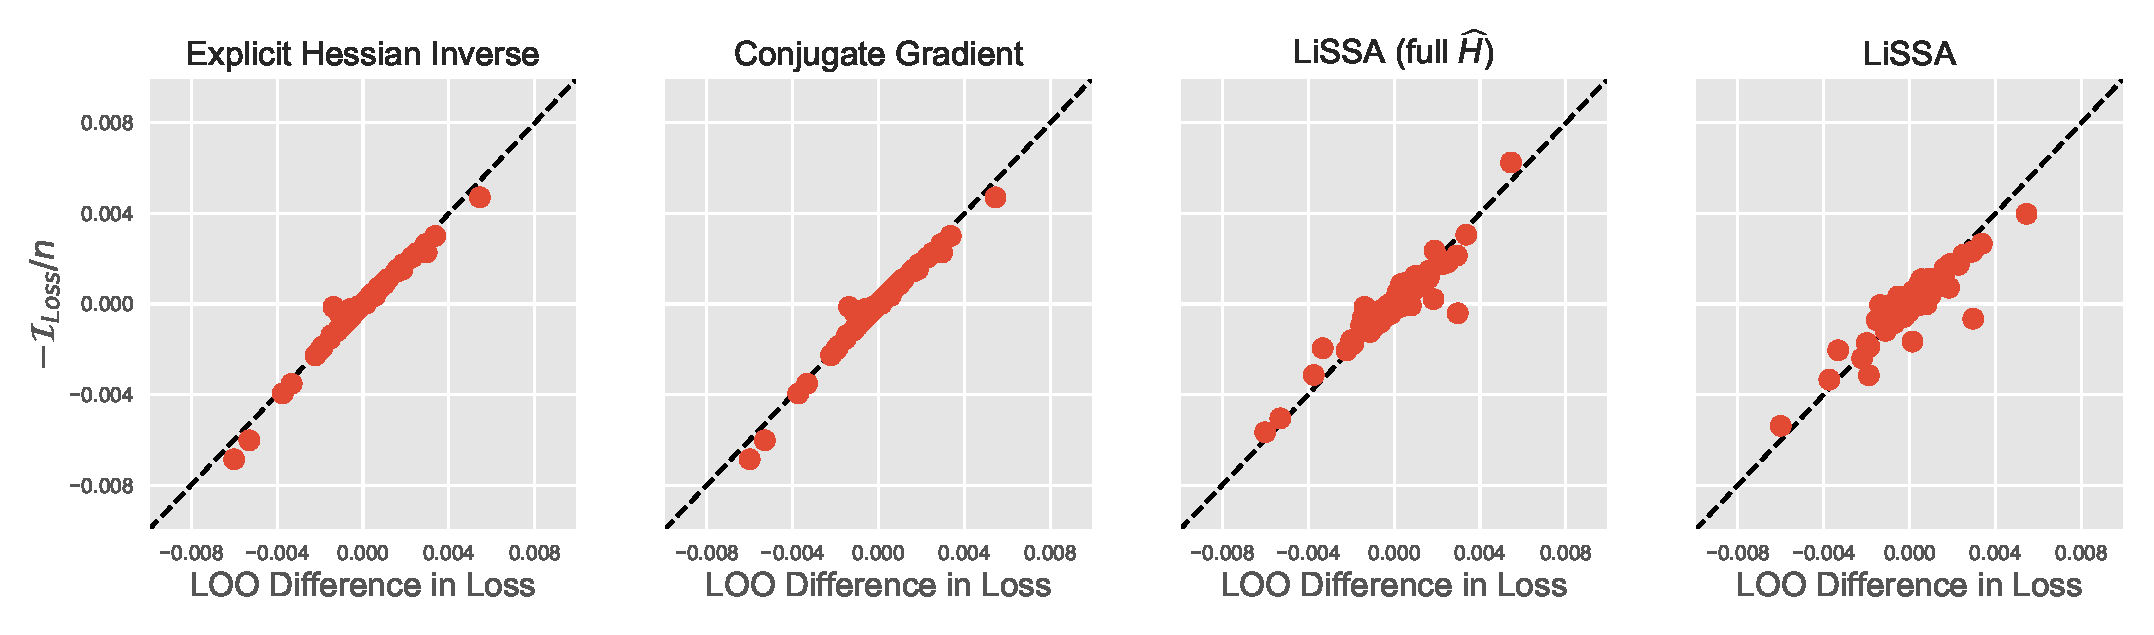
\includegraphics[width=2.1\columnwidth]{fig-ridge}}
\vskip -0.1in
\caption{\textbf{Influence function} $\mathcal{I}_{\mathcal{L}}(\bm{z}_{tr}, \bm{z}_{te})$ \textbf{matches leave-one-out difference.} We randomly picked a validation point $\bm{z}_{te}$ and calculated the influence on validation loss for all training points $\bm{z}_i$. In this illustration $\bm{z}_{te}$ is the $42^{\text{rd}}$ instance in the dataset, and $\mathcal{I}_{\mathcal{L}}$ was evaluated for the rest 516 points. \textbf{(Panel-1):} We plotted the LOO difference $\mathcal{L}(\bm{z}_{te}, \fixwidehat{\bm{\theta}}_{-\frac{1}{n},\bm{z}_i})$ $- \mathcal{L}(\bm{z}_{te}, \fixwidehat{\bm{\theta}})$ against $-\frac{1}{n}\mathcal{I}_{\mathcal{L}}(\bm{z}_{i}, \bm{z}_{te})$ for each $\bm{z}_i$. The influence is calucated by explicitly forming and inverting hessian matrix $\nabla_{\bm{\theta}}^2 R(\fixwidehat{\bm{\theta}})$. \textbf{(Panel-2):} The influence is evaluated by solving the linear system with conjugate gradients, only hessian-vector products were evaluated. \textbf{(Panel-3):} The influence was evaluated with the original Taylor approximation. The recursion step is \emph{exactly} the same as (\ref{lissarule}), i.e. the HVPs were evaluated with the \emph{full} empirical risk $R(\fixwidehat{\bm{\theta}})$. We set the recursion depth to be $m=2000$, and we divided the HVPs by a scaling constant $C=400$ to ensure the convergence of the power series. \textbf{(Panel-4):} The influence was evaluated with the LiSSA algorithm: for each recursion step, the algorithm only look at one training point $\bm{z}_j$, and the HVP was evaluated with that \emph{single} element of loss $\mathcal{L}(\bm{z}_j, \fixwidehat{\bm{\theta}})$. We used the same recursion depth and scaling constant.} 
\label{ridge_examples}
\end{center}
\vskip -0.25in
\end{figure*} 
We fit a ridge regression with $\lambda = 1.0$ on the \href{https://archive.ics.uci.edu/ml/datasets/forest+fires}{\texttt{ForestFires}} dataset, a regression task with 517 instances and 13 features. The aim is to predict the burned area of forest fires. We randomly draw a validation point and use the rest instances to fit the model. 

After training the model, we computed $\mathcal{L}(\bm{z}_{te}, \fixwidehat{\bm{\theta}}_{-\frac{1}{n},\bm{z}_i})$ $- \mathcal{L}(\bm{z}_{te}, \fixwidehat{\bm{\theta}})$, the difference between the validation loss after doing actural LOO retaining and the original loss with $\fixwidehat{\bm{\theta}}$, for all training points. Then, we plot the actual LOO difference against its asymptotic approximation, $-\frac{1}{n}\mathcal{I}_{\mathcal{L}}(\bm{z}_{tr}, \bm{z}_{te})$, to assess the accuracy of our influence functions with all three methods that we discussed: explicit hessian inverse, conjugate gradients, and stochastic Taylor approximation (LiSSA). The results are presented in Figure \ref{ridge_examples}. 

The influence and the leave-one-out difference matches chosely. For explicit hessian inverse and CG, there was an almost exact match. For Taylor approximation methods, there was a little variance; furthermore, we didn't lose much accuracy when switching from full HVP to LiSSA algorithm, but increased the speed by $n$ times.

\subsection{Logistic Regression}
Next we switch to classification tasks. A closed-form expression of $\mathcal{I}_{\mathcal{L}}(\bm{z}_{tr}, \bm{z}_{te})$ is also easy to derive for the logistic regression empirical risk. Let $\sigma(t)=1/(1+e^{-t})$, label $y\in \{0,1\}$, we have
\begin{align}\label{logit_R}
\vspace{-0.2in}
R_{\text{logit}}(\fixwidehat{\bm{\theta}}) = \frac{1}{n}\sum_{i=1}^n \left(-y_i\fixwidehat{\bm{\theta}}^{\top}\bm{x}_i + \log(1+e^{\fixwidehat{\bm{\theta}}^{\top} \bm{x}_i})\right)
\vspace{-0.2in}
\end{align}
For a certain validation point, the loss is $\mathcal{L}(\bm{z}_{te}, \fixwidehat{\bm{\theta}}) = -y\fixwidehat{\bm{\theta}}^{\top}\bm{x}_{te} + \log(1+e^{\fixwidehat{\bm{\theta}}^{\top} \bm{x}_{te}})$. Hence the influence of a training point $\bm{z}_{tr}$ on that validation loss is:
\begin{align}\label{logit_I_loss}
\vspace{-0.15in}
\mathcal{I}_{\mathcal{L}_{logit}}(\bm{z}_{tr}, \bm{z}_{te}) &= -\bm{x}_{tr}^{\top}\nabla_{\bm{\theta}}^2 R(\fixwidehat{\bm{\theta}})^{-1} \bm{x}_{te}\cdot\\
&(\sigma(\fixwidehat{\bm{\theta}}^{\top}\bm{x}_{tr})-y_{tr})(\sigma(\fixwidehat{\bm{\theta}}^{\top}\bm{x}_{te})-y_{te})\notag\\[-3pt]
\nabla_{\bm{\theta}}^2 R(\fixwidehat{\bm{\theta}})&=\frac{1}{n}\sum_{i=1}^n \sigma(\fixwidehat{\bm{\theta}}^{\top}\bm{x}_i)\sigma(-\fixwidehat{\bm{\theta}}^{\top}\bm{x}_i)\bm{x}_i\bm{x}_i^{\top}\notag
\vspace{-0.15in}
\end{align}
If there is an $L_2$-regularization, we just need to fold the $\frac{\lambda}{n} \left\lVert \fixwidehat{\bm{\theta}}\right\rVert_2^2$ into the loss function like we did for the Ridge regression. 

\cite{koh2017} discussed an alternative formulation of logistic loss. Instead of using 0-1 labels, consider $y \in \{1,-1\}$. The loss function under this $\pm 1$ formulation is the loss is $\mathcal{L}(\bm{z}_{te}, \fixwidehat{\bm{\theta}}) = \log(1+e^{-y_{te}\fixwidehat{\bm{\theta}}^{\top} \bm{x}_{te}})$. The influence of a training point on that $\pm1$ validation loss is:
\begin{align}\label{logit_I_loss2}
\vspace{-0.15in}
\mathcal{I}'_{\mathcal{L}_{logit}}(\bm{z}_{tr}, \bm{z}_{te}) &= -\bm{x}_{tr}^{\top}\nabla_{\bm{\theta}}^2 R(\fixwidehat{\bm{\theta}})^{-1} \bm{x}_{te}\cdot\\
&y_{tr}\sigma(-y_{tr}\fixwidehat{\bm{\theta}}^{\top}\bm{x}_{tr})\cdot y_{te}\sigma(-y_{te}\fixwidehat{\bm{\theta}}^{\top}\bm{x}_{te})\notag
\vspace{-0.15in}
\end{align}
One can examine that (\ref{logit_I_loss}) and (\ref{logit_I_loss2}) are equivalent. 


\begin{figure*}[ht]
\vskip 0.0in
\begin{center}
\centerline{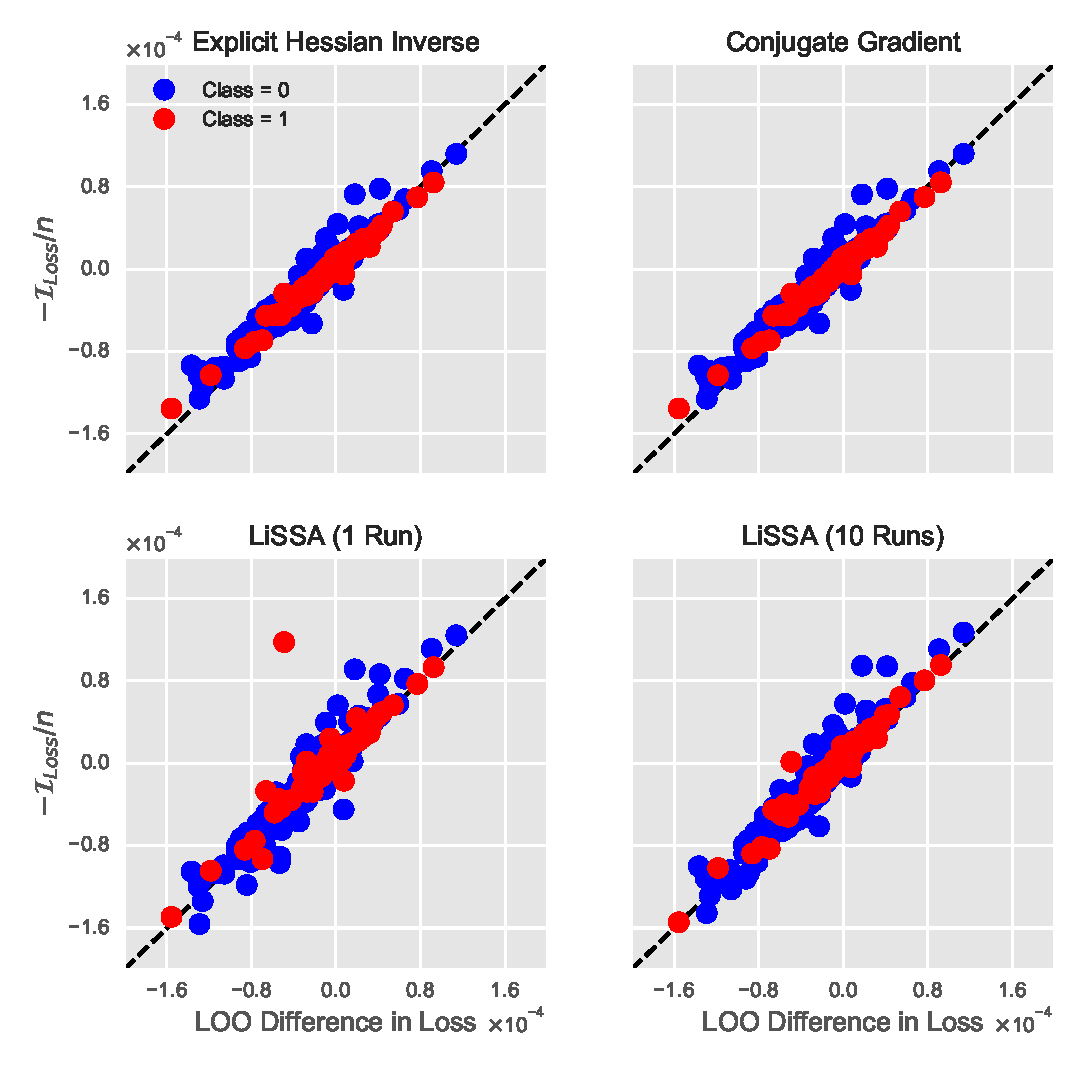
\includegraphics[width=1\columnwidth]{fig-logit}
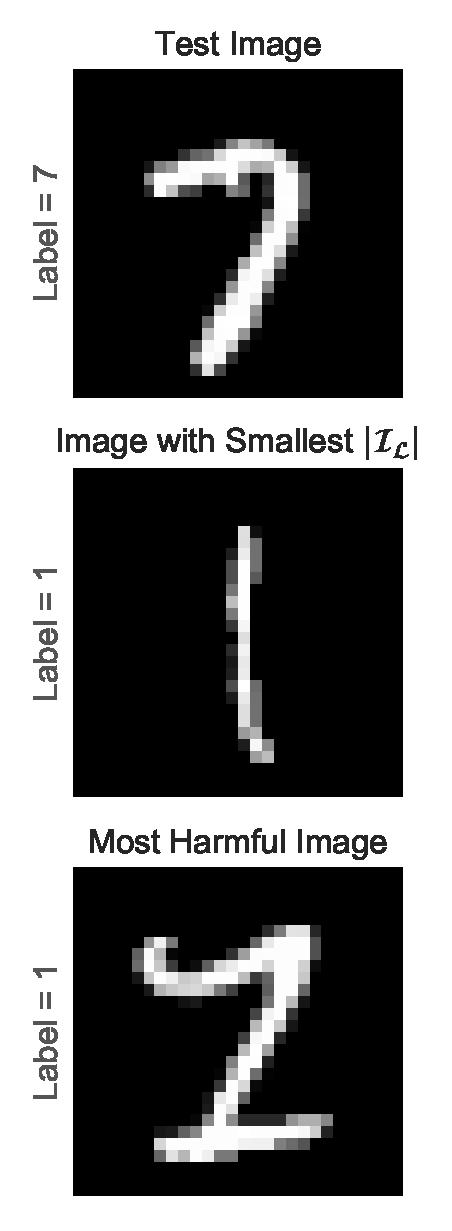
\includegraphics[width=0.35\columnwidth]{fig-logit-img}}
\vskip -0.1in
\caption{\textbf{Influence for handwritten digits classification.} In this illustration $\bm{z}_{te}$ is the $7^{\text{th}}$ instance in the dataset. The red dots stand for positive points, blue for negative points. \textbf{(Left):} We plotted the LOO difference $\mathcal{L}(\bm{z}_{te}, \fixwidehat{\bm{\theta}}_{-\frac{1}{n},\bm{z}_i})$ $- \mathcal{L}(\bm{z}_{te}, \fixwidehat{\bm{\theta}})$ against $-\frac{1}{n}\mathcal{I}_{\mathcal{L}}(\bm{z}_{i}, \bm{z}_{te})$ for all the three methods. The explicit hessian inverse and the CG method are the same as we used in the Ridge experiment. For the LiSSA method we sampled 1 training point in each recursion step, and we set the recursion depth as $m=10000$; we divided the HVPs by a scaling constant $C=10^3$. An outlier can be observed in the Southwest panel where we ran the LiSSA algorithm only once. In the Southeast panel, we ran the algorithm 10 times, and took average to obtain the final estimate. The variance is reduced and the outlier has gone. \textbf{(Right):} The upper panel shows the validation point. The middle panel is the training point with the smallest influence, i.e. the smallest $| \mathcal{I}_{\mathcal{L}}(\bm{z}_{i}, \bm{z}_{te}) |$. It looks like an ``easy'' positive point. The bottom panel is the training point with the largest negative influence, which looks like a ``hard'' positive point. It can be thought as the most harmful to predicting $\bm{z}_{te}$ in the sense that removing this point will cause reduce the prediction loss.} 
\label{logit_examples}
\end{center}
\vskip -0.3in
\end{figure*} 

We fit an $L_2$-regularized logistic regression model with $\lambda = 1000$ on the \href{http://yann.lecun.com/exdb/mnist/}{\texttt{MNIST}} dataset. For simplicity we only include digits 1 and 7, and we let the label $y=1$ stand for digit 1 and $y=0$ for digit 7. The resulting binary MNIST dataset has 9084 instances; each instance is a $28\times 28$ image, represented by grayscale matrix. We first standardize the data before training the model, it turns out that standardizing helps control the numerical scale of losses, and stabilizes the influence calculation. Then, we randomly choose a testing point and calculate the influence of the rest training points; we also compute the actual LOO difference using \texttt{sklean}'s LBFGS solver. The results are presented in Figure \ref{logit_examples}. Note that there are points from both classes that have positive or negaive influences, indicating that $\text{sgn}(\mathcal{I}_{\mathcal{L}}(\bm{z}_{i}, \bm{z}_{te}))$ is \emph{not} determined by whether $y_{te}=y_{tr}$ or not.

On \href{http://yann.lecun.com/exdb/mnist/}{\texttt{MNIST}} dataset, we performed another analysis on the closed-form expression (\ref{logit_I_loss2}): we examined the effect of the $\sigma(-y_{tr}\fixwidehat{\bm{\theta}}^{\top}\bm{x}_{tr})$ factor and the hessian matrix on the influence. The analysis is shown in Figure \ref{logit_components}. In particular, we replicated the approach in the original paper by plotting $\mathcal{I}_{\mathcal{L}}(\bm{z}_{tr}, \bm{z}_{te})$ calculated by (\ref{logit_I_loss2}) against its variants that misses certain factor(s). 

\setcounter{figure}{3}
\begin{figure*}[h]
\vskip 0.0in
\begin{center}
\centerline{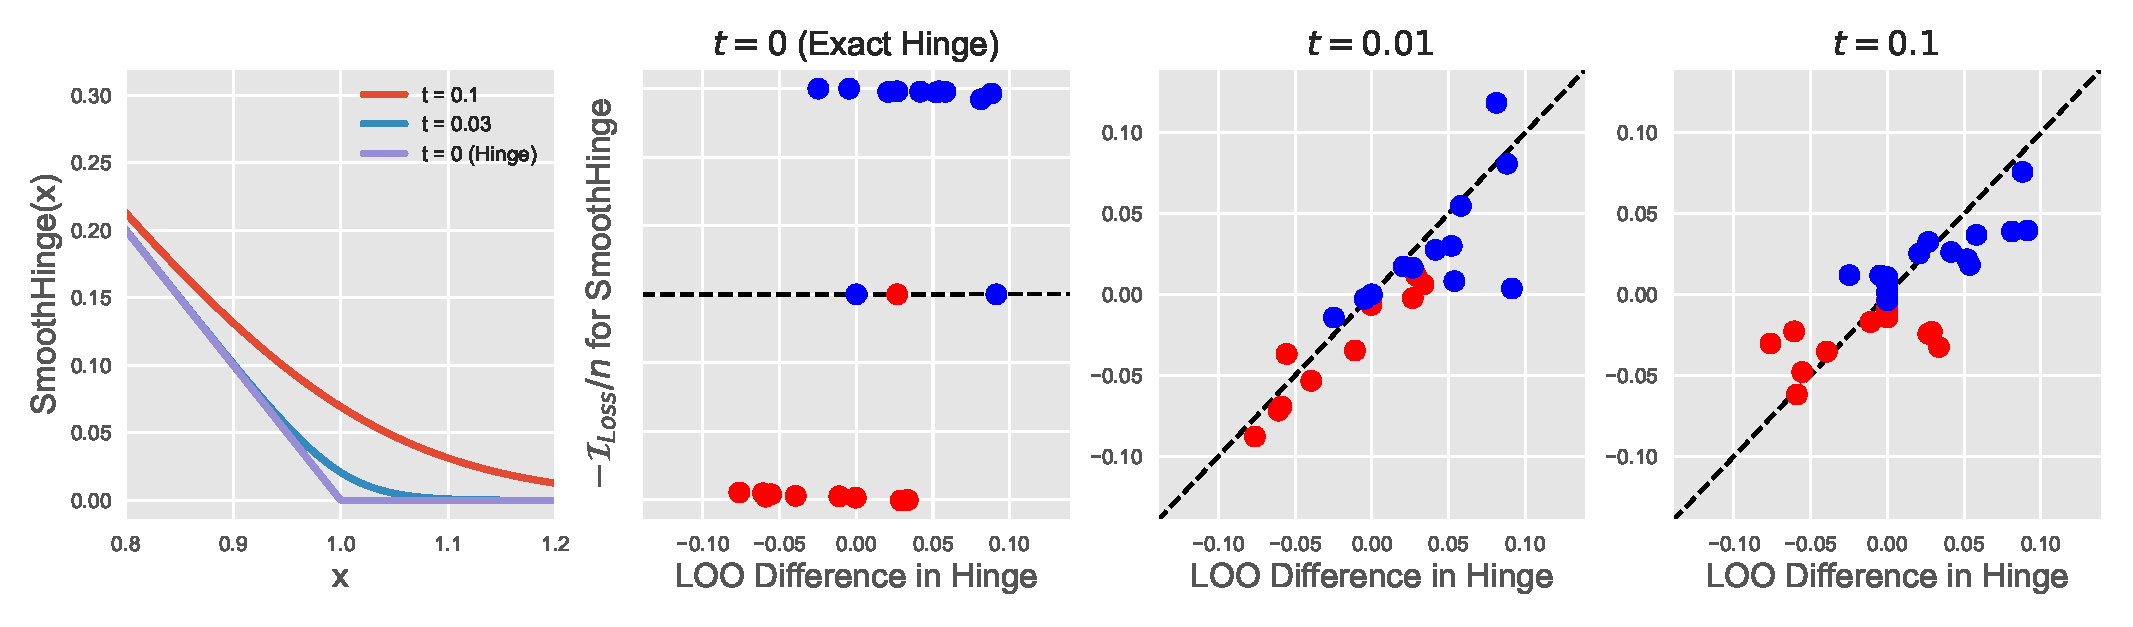
\includegraphics[width=2.1\columnwidth]{fig-svm}}
\vskip -0.1in
\caption{\textbf{Smooth approximation to the non-differentiable loss.}  In this illustration, the red dots stand for $y=1$ points, blue for $y=-1$ points. The influence calculated with \emph{smoothed} hinge loss is plotted on y-axis, while the LOO difference in exact hinge loss ($t=0$) is plotted on x-axis. The black-dashed line has slope 1. \textbf{(Panel-1):} By varying $t$, we can approximate the hinge loss with arbitrary accuracy. \textbf{(Panel-2):} We force the system to compute $\mathcal{I}_{\mathcal{L}}(\bm{z}_{tr}, \bm{z}_{te})$ for the $t=0$ non-differentiable case. The influence function is not a good estimate of LOO difference, overestimating it disastrously. The is due to the fact that $\nabla^2 R_{\text{sv}}(\fixwidehat{\bm{\theta}})$ is close to zero in this setting, providing no information to the quadratic approximation of $\mathcal{L}(\bm{z}, \fixwidehat{\bm{\theta}})$. As a result, the quadratic approximation is linear, leading to overestimating the true influence. \textbf{(Panel-3):} The influence is computed for the smoothed empirical risk with $t=0.01$. The correlation coefficient between $\mathcal{I}_{\mathcal{L}}(\bm{z}_{tr}, \bm{z}_{te})$ and hinge LOO difference is $0.8602$. \textbf{(Panel-4):} $t=0.1$, correlation is $0.7700$. With $t$ too large, the smoothed loss is no longer a good approximation of the original hinge loss, so the correlation decreases.}
\label{smoothsvm}
\end{center}
\vskip -0.25in
\end{figure*}

\setcounter{figure}{2}
\begin{figure}[H]
\vskip 0.0in
\begin{center}
\centerline{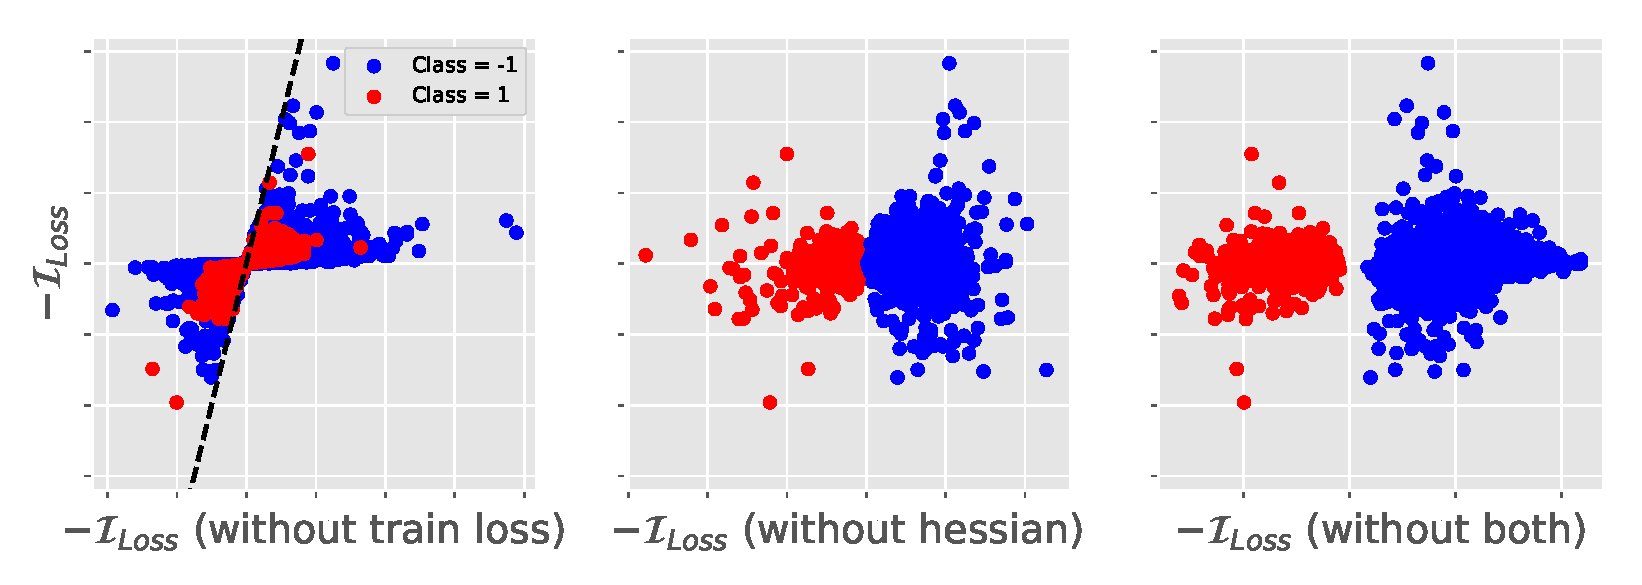
\includegraphics[width=\columnwidth]{fig-components}}
\vskip -0.1in
\caption{\textbf{Components of influence.} The correct influence is plotted on y-axis, while its variants that misses certain factor(s) are plotted on x-axis. Blue dots are the training points with \emph{same label} as $\bm{z}_{te}$; red dots are the opposites. \textbf{(Left):} The black-dashed line has slope = 1; one can observe that many points lie to the right of the $45^{\circ}$ line in the first quadrant, suggesting that we overestimate the influence of these training points if the factor $\sigma(-y_{tr}\fixwidehat{\bm{\theta}}^{\top}\bm{x}_{tr})$ was excluded. \textbf{(Mid):} Without the hessian inverse, $\text{sgn}(\mathcal{I}_{\mathcal{L}}(\bm{z}_{i}, \bm{z}_{te})) = \bm{1} (y_{te}=y_{tr})$. This is due to the fact that we used the unscaled data, where all features are positive grayscales. Clearly, this is incorrect since we have illustrated in Fugure \ref{logit_examples} that points from both classes can be helpful or harmful. \textbf{(Right):} Without both factors, the influence degenerates into $\bm{x}_{tr}^{\top} \bm{x}_{te}\cdot [y_{tr}y_{te}\sigma(-y_{te}\fixwidehat{\bm{\theta}}^{\top}\bm{x}_{te})] = \bm{x}_{tr}^{\top} \bm{x}_{te}c$, which is just the inner product scaled by a constant. } 
\label{logit_components}
\end{center}
\vskip 0in
\end{figure}


\subsection{Support Vector Machine}
Until now, we have assumed that the loss function is twice differentiable. However, non-differentiable losses, such as hinge loss and $L_1$ regularization, are common in statistical learning. The idea to make things work is to construct a smooth function that converges to the non-differentiable components of the loss function. Then, we minimize the smoothed version of the empirical risk, and compute $\mathcal{I}_{\mathcal{L}}(\bm{z}_{tr}, \bm{z}_{te})$. In this section, we examplify this general idea with the linear support vector classifier. Besides, we show that the influence computed for the smoothed linear SVC is still a good approximation to the LOO difference.

For a binary classification problem with label $y\in\{1,-1\}$, the linear SVC hypothesis is parametrized by weights and intercept: $\bm{\theta} = (\bm{\beta}, \beta_0)$, and the empirical risk is, by \cite{ESL}:
\begin{align}\label{svc_R}
\vspace{-0.2in}
R_{\text{sv}}(\fixwidehat{\bm{\theta}}) = \frac{1}{n}\sum_{i=1}^n \left[h\left(y_i(\bm{x}_i^{\top} \fixwidehat{\bm{\beta}} + \fixwidehat{\beta_0})\right) + \frac{\lambda}{2n} \left\lVert \bm{\beta}\right\rVert_2^2\right]
\vspace{-0.2in}
\end{align}
Where $h(x) = \max\{0, 1-x\}$ is the hinge loss. \cite{koh2017} constructed a smooth approximation of $h$. Let $t>0$ be a constant hyperparameter, define $h_t(x) := t\log(1+\text{exp}(\frac{1-x}{t}))$, one can show that $h_t$ converges to $h$ as $t\to 0$. (See Figure \ref{smoothsvm} Panel-1). Therefore, we replace the hinge function in (\ref{svc_R}) with $h_t$, and examine the influence induced by the hessian matrix of this smoothed empirical risk.

We fit a smoothed linear SVC with $\lambda = 2.0$ on the classic \href{https://archive.ics.uci.edu/ml/datasets/iris}{\texttt{Iris}} dataset. For simplicity we only include two classes: $y=1$ for \emph{Versicolor}, and $y=-1$ for \emph{Virginica}. The resulting binary Iris dataset has 100 instances and 4 features. We start by randomly choosing 10 testing points, fit the smoothed linear SVC, and calculate the influence of the rest training points with (\ref{svc_R}). Then, we compute the actual LOO difference using the original hinge loss ($t=0$). The results are presented in Figure \ref{smoothsvm}. 


\section{Applications}
The influence function can be applied in many real-life cases, and can help us get a better understanding upon how black-box models rely on and extrapolate from the training data. \cite{koh2017} discussed different use cases of influence functions, including adversarial training (training set attacks), debugging domain mismatch, and fixing mislabeled examples.

In this section, we perform an additional experiments to exemplify the applications of influence functions: We uncover the difference of two hyperplane classifiers and understand their behaviors with the help of influence function. 

\subsection{Understanding Model Behavior}
Two models can make the same correct predictions and achieve similar level of performance, but get there in very different ways. Binary logistic regression and linear support vector classifier are very simple models. They can be both regarded as a separating hyperplane that tries to cut the high-dimensional data into two classes. Nevertheless, they have very different behaviors and interpretations. This difference is, indeed, a direct result from the different mathematical form of the loss functions. Therefore, looking at $\mathcal{I}_{\mathcal{L}}(\bm{z}_{tr}, \bm{z}_{te})$ of both models for the same dataset can give us an intuitive picture in terms of how the two mathematical form of $\mathcal{L}(\bm{z}, \fixwidehat{\bm{\theta}})$ trace back to the same training data in different ways.

For our purpose, we train the logistic regression and linear SVC on the same \href{https://archive.ics.uci.edu/ml/datasets/iris}{\texttt{Iris}} dataset, and compute $\mathcal{I}_{\mathcal{L}}(\bm{z}_{tr}, \bm{z}_{te})$ for \emph{the same} testing point. By plotting the influence against the Euclidean distance to the decision boundary (see Figure \ref{model_behav_fig}), we found the two models behave differently in terms of how the training data are used for prediction: Both models put more leverage on the points that are closer to the separating hyperplane. However, logistic regression looks at more points; while linear SVC \emph{does not} look at points that are too far away from the boundary: those points have zero influence on testing loss.

\setcounter{figure}{4}
\begin{figure}[h]
\vskip 0.0in
\begin{center}
\centerline{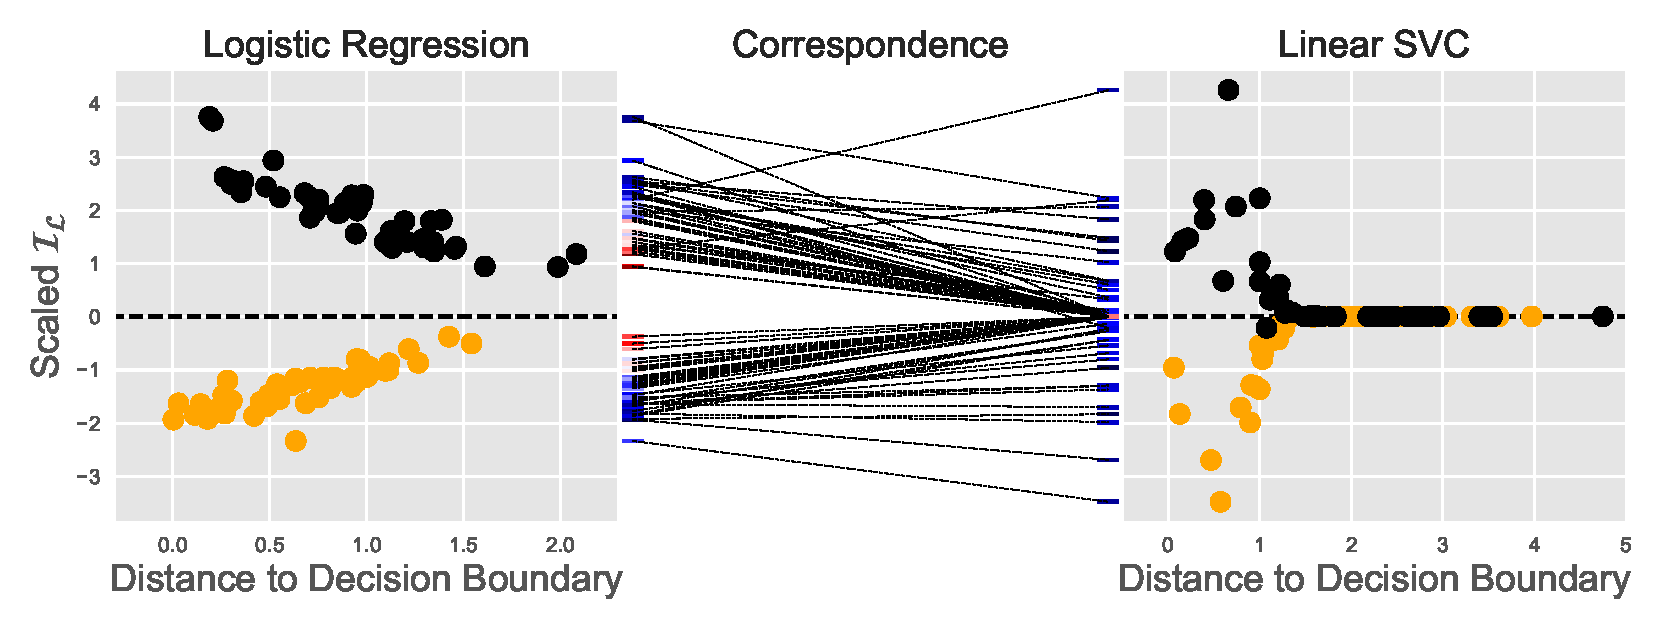
\includegraphics[width=\columnwidth]{fig-app1}}
\vskip -0.1in
\caption{\textbf{Logistic regression V.S. Linear SVC.} We compare the behavior of logistic regression and linear SVC for the same testing point. For each training point $\bm{z}_{i}$, $\mathcal{I}_{\mathcal{L}}(\bm{z}_{i}, \bm{z}_{te})$ is plotted on y-axis; while $ (\bm{x}_{i}^{\top}\fixwidehat{\bm{\beta}}+\beta_0) / \left\lVert \fixwidehat{\bm{\beta}}\right\rVert$, the Euclidean distance to the decision boundary is plotted on x-axis. \textbf{(Left):} For logistic regression, the absolute value of influence decreases slowly for points that are further away from the boundary, and it's always non-zero. \textbf{(Mid):} The thin dashed line connects the same training point in the two settings; the ticks on y-axis mark the influence level of that particular training point; the color of ticks stand for distance to the boundary: blueish for close, redish for faraway. \textbf{(Right):} For linear SVC, the influence decrease much faster, and those training points that are far beyond the margin have literally zero influence.} 
\label{model_behav_fig}
\end{center}
\vskip 0in
\end{figure}


\section{Software Package}
We built a generic empirical risk optimizing framework with \texttt{Tensorflow} to compute influence functions for various models, and we also implemented CG and LiSSA algorithm to scale up to large datasets. With the help of auto-gradients system, the required gradients and hessian-vector products are automatically kept track of. The user only need to define the empirical risk funtion and its parametrization. All of our code, data, and reproducible experiments are available in our \href{https://github.com/zedyang/46927-Project}{Github repository}.



\bibliography{report}
\bibliographystyle{icml2017}

\end{document} 


% This document was modified from the file originally made available by
% Pat Langley and Andrea Danyluk for ICML-2K. This version was
% created by Lise Getoor and Tobias Scheffer, it was slightly modified  
% from the 2010 version by Thorsten Joachims & Johannes Fuernkranz, 
% slightly modified from the 2009 version by Kiri Wagstaff and 
% Sam Roweis's 2008 version, which is slightly modified from 
% Prasad Tadepalli's 2007 version which is a lightly 
% changed version of the previous year's version by Andrew Moore, 
% which was in turn edited from those of Kristian Kersting and 
% Codrina Lauth. Alex Smola contributed to the algorithmic style files.  
